\documentclass[11pt,letterpaper]{exam}
%\usepackage[Lhdr={},Rhdr={}]{plain}

\usepackage{tikz}
\usetikzlibrary{shapes.geometric}
\usepackage{pgfplots}
\usepackage{verbatim}
\usepackage{comment}
\usepackage{graphicx}
\usepackage{multicol}
\usepackage{mathtools}
\usepackage[table,xcdraw]{xcolor}
\usepackage[top=0.5in,
  headsep=0pt% remove space between header and text body
  ]{geometry}
\usepackage{lastpage}
\cfoot{Page \thepage \hspace{1pt} of \pageref{LastPage}}

\newcommand{\figpath}{figs/}

\usepackage{titlesec}
\titleformat*{\section}{\large\bfseries}

% These are my colors -- there are many like them, but these ones are mine.
\definecolor{blue}{RGB}{0,114,178}
\definecolor{red}{RGB}{213,94,0}
\definecolor{yellow}{RGB}{240,228,66}
\definecolor{green}{RGB}{0,158,115}
\newcommand{\blue}[1]{\textcolor{blue}{#1}}
\newcommand{\red}[1]{\textcolor{red}{#1}}


\begin{document}


\begin{center}

{\large

\textbf{Midterm Exam\\International Trade Theory and Policy\\Fall 2025}

}
\end{center}

\section*{Part I: True or False (10 points)}

\begin{questions}
\question In the Ricardian model, countries can gain from trade even if one country is more productive in producing every good.

\red{True. Gains from trade arise due to comparative advantage, not absolute advantage.}

\question When there are multiple active sectors that use labor in a country and labor is a freely mobile factor across sectors, each sector will pay a different wage.

\red{False. If multiple active sectors and labor is mobile, the wage is equalized across sectors. Otherwise, all labor would move to the sector that pays the highest wage and a single sector would be active.}

\question Let a production function be defined as $F(K) = K^{1/3}$. This production function has the property of marginal decreasing capital.

\textcolor{red}{True. It is decreasing returns to capital. Let $\lambda > 1$. Then:}

\begin{eqnarray*}
    \textcolor{red}{
        F(\lambda K)} &=& \textcolor{red}{(\lambda K)^{1/3}} \\
        &=& \textcolor{red}{\lambda^{1/3} K^{1/3}} \\
        &=& \textcolor{red}{\lambda^{1/3} F(K) < \lambda F(K)
    }
\end{eqnarray*}

\question In the Ricardian model, the opportunity cost of producing one good in terms of the other is constant.

\red{True. The Ricardian model assumes a linear technology with a single factor of production (labor) with constant returns to scale.  As a consequence, the PPF is linear and the opportunity cost of producing one good in terms of the other is  constant.}

\question In the Specific Factors model, the opportunity cost of producing one good in terms of the other is constant.

\red{False. The Specific Factors model assumes a Cobb-Douglas technology. Since one of the factors is supplied in fixed proportion, labor has decreasing marginal returns to scale. As a consequence, the PPF is concave and the opportunity cost of producing one good in terms of the other is not constant.}

%\question In the production model, the firm chooses prices to maximize profits.

%\textcolor{red}{False. In the production model, the firm takes prices as given and chooses $K,L$ to maximize profits.}

%\question The fact that scientific models have some unrealistic assumptions is necessarily a problem.

%\red{False. The fact that models simplify the world is a feature not a bug in scientific models. They do away with aspect os reality so we can focus on a particular causal mechanism.}

\question In the Specific Factors Model, capital can be instantly moved between agriculture and manufacturing.

\red{False. Capital is specific to manufacturing; it is not mobile between sectors in the short run.}

\question Trade openness is associated with higher GDP per capita across countries.

\red{True. The empirical relationship is positive on average, as we saw in class.}

%\question Everybody gains from trade.

%\red{False. Even though trade tends to increase aggregate income (GDP) there will be winners and losers, especially over the short run.}

\question In the Specific Factors Model, owners of the specific factor in the export sector gain from trade.

\red{True. The price of your production increases, and so does your return.}

\question Empirical evidence shows that most US workers benefited from trade integration with China.

\red{True. As we saw in class, real wages increased for about 94\% of workers due to lower import prices.}

\question Empirical evidence shows that all US workers benefited from trade integration with China.

\red{False. Some workers and firms faced losses from Chinese import competition and were displaced out of the market.}

\end{questions}

\section*{Part II: Multi-Part Problems (90 points)}

\begin{questions}

\question[45]  Consider the Two-Country, Two-Goods Ricardian model that we have studied in class. There are two countries $i \in \{ US,COL \}$ and two products $p \in \{R,C \}$.

In each country, there is a representative household with preferences over the consumption of each good $Q_{i,p}$ denoted by an utility function $U_{i}(Q_{i,R} , Q_{i,C})$, taking goods prices $P_{p}$ as given. They supply labor $L_i$ inelastically for wage $w_i$. Suppose that consumer preferences are Cobb-Douglas with weight $0 < \alpha_i < 1$ on roses. 

Markets for each product in each country are competitive and firms maximize profits by choosing optimal production $Y_{i,p}$ levels, taking goods $P_{p}$, unit labor requirements $a_{i,p}$ and factor $w_i$ prices as given.  

Total labor allocation in this economy satisfies $L_i = a_{i,R} Y_{i,R} + a_{i,C} Y_{i,C}$.

\begin{parts}
\part[5]  Focus on the United States ($i= US$). State the demand functions for each good as a function of parameters $\{\alpha_{US}, 1-\alpha_{US}\}$, income $w_{US}L_{US}$ and prices $\{P_R,P_C\}$ (you do not have to solve for it, just state them); are these functions increasing or decreasing in prices? -- explain the intuition. 

\red{
Demand functions are:
}
\red{
\begin{equation*} 
    Q_{US,R} = \alpha_{US} \frac{w_{US} L_{US}}{P_R}, \qquad Q_{US,C} = (1-\alpha_{US}) \frac{w_{US} L_{US}}{P_C}
\end{equation*}
 }
 \red{
They are decreasing in prices, since demand curves slope down (the higher the price, the lower the demand).
}
\part[5] Write down the profit maximization problem for a firm in the US producing product $p$.


\textcolor{red}{
\begin{equation*} 
    \max_{Y_{US,p}} \pi_{US,p} = P_{US,p} Y_{US,p} - w_{US} a_{US,p} Y_{US,p}  
\end{equation*}
}

\part[5] In competitive markets, there is no economic profit, so prices equal marginal cost. Derive this condition from the problem above.

\textcolor{red}{
\begin{equation*} 
    \pi_{US,p} = P_{US,p} Y_{US,p} - w_i a_{US,p} Y_{US,p} = 0 \implies P_{US,p} = w_i a_{US,p} 
\end{equation*}
}

\part[5] Suppose $a_{i,C} = 2$ and $a_{i,R} = 4$. Calculate relative prices $P_{R}/P_{C}$.

\textcolor{red}{
\begin{equation*} 
    \frac{P_{US,p}}{a_{US,p}} = w_{US}  \text{ for each }p \implies \frac{P_{C}}{a_{US,C}}=\frac{P_{R}}{a_{US,R}} \iff \frac{P_{R}}{P_{C}}=\frac{a_{US,R}}{a_{US,C}} = 2
\end{equation*}
}

\part[10] Suppose $L_{i} = 10$. Using the labor allocation constraint, draw the production possibilities frontier on the $(Y_{US,R}, Y_{US,C})$ space. (5 pts) Make sure to draw all the labels and edge points (where your PPF intersects with each of the axes) correctly; and (5 pts) explain the relation between the slope of the PPF and your result in the previous part.

\begin{tikzpicture}
\pgfmathsetmacro{\aC}{2}       % unit labor requirement for computers
\pgfmathsetmacro{\aR}{4}         % unit labor requirement for roses
\pgfmathsetmacro{\Lendow}{10}    % labor endowment


\centering
\begin{axis}[
    ylabel={Quantity of computers, $ \textcolor{blue}{Y_{US,C}}$},
    xlabel={Quantity of roses, $\textcolor{blue}{Y_{US,R}}$},
    ymin=0, ymax=6,
    xmin=0, xmax=6,
    yticklabel=\empty,
    xticklabel=\empty,
    axis lines=left,
    enlargelimits=false,
    clip=false,
    axis on top,
    scaled x ticks=false,
    width=9cm, height=7cm,
    title style={font=\bfseries}
]

% PPF: Q_C = (L/a_C) - (a_R/a_C) * Q_R
\addplot[thick, blue, domain=0:5/2] {\Lendow/\aC - (\aR/\aC)*x};

% Indifference curve through optimal bundle
%\addplot[red, domain=0.1:9, samples=100] {\A * x^(-\expo)};

% Labels

%\node at (axis cs:3.5,0.03) {\Large $\mathcal{Y}_{US}$};
\node at (axis cs:\Lendow/\aR,-.4) {\scriptsize $5/2$};
\node at (axis cs:-.4,\Lendow/\aC) {\scriptsize $5$};


\end{axis}

\end{tikzpicture}
\red{
\\The slope of this curve is $-a_{US,R}/a_{US,C}= -P_{US,R}/P_{US,C}=-2$ denotes relative prices. To see that, start from the resource constraint and solve it for $Y_{US,C}$ (the y axis on the chart above):
}
\red{
\begin{eqnarray*}
    L_{US} &=& a_{US,R} Y_{US,R} + a_{US,C} Y_{US,C} \\
    \iff a_{US,C} Y_{US,C} &=&  L_{US} - a_{US,R} Y_{US,R} \\ 
    \iff  Y_{US,C} &=& \frac{ L_{US} }{a_{US,C}} - \frac{a_{US,R}}{a_{US,C}} Y_{US,R} \\ 
    \iff  Y_{US,C} &=& \frac{ L_{US} }{a_{US,C}} - \frac{P_{US,R}}{P_{US,C}} Y_{US,R} \
\end{eqnarray*}
}
\part[5] Now imagine that, after opening up to trade, relative prices change to $P_R / P_C = 1 < 2$. (5 pts) Would the US specialize in the production of computers or roses? 
\red{
Roses are now relatively cheap and computers relatively expensive at world prices compared to autarky prices. Therefore, the U.S. will specialize in the production of computers, exporting them in exchange for imported roses.
}
\part[10] Using the information above, draw a chart of US production consumption after trade where you plot (i) the PPF; (ii) the world price line; (iii) a point $Y$ denoting production; (iv) and the indifference curve at some point along the world price line. 


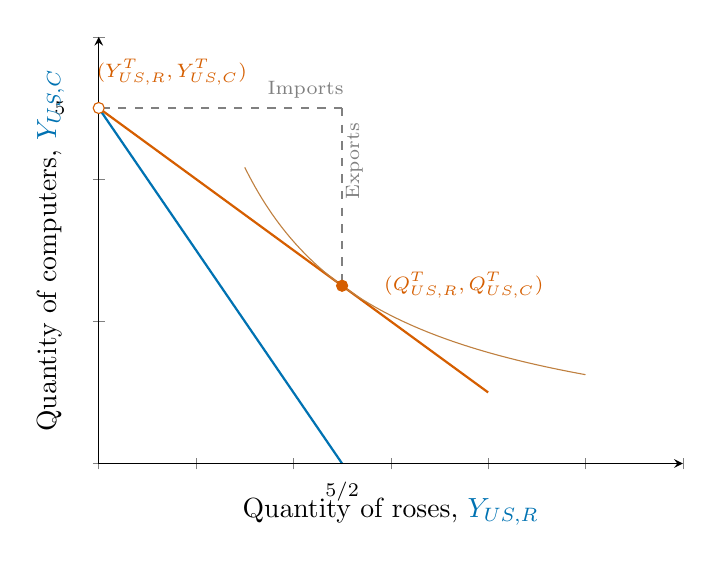
\begin{tikzpicture}
\pgfmathsetmacro{\aC}{2}       % unit labor requirement for computers
\pgfmathsetmacro{\aR}{4}         % unit labor requirement for roses
\pgfmathsetmacro{\Lendow}{10}    % labor endowment
\pgfmathsetmacro{\p}{1}    % price under trade
\pgfmathsetmacro{\alpha}{1/2}    % price under trade
% Compute equilibrium quantities
\pgfmathsetmacro{\QcT}{(\alpha*\Lendow)/\aC}
\pgfmathsetmacro{\QrT}{((1 - \alpha)*\p*\Lendow)/\aC}
% Compute utility level
\pgfmathsetmacro{\UT}{(\QcT^(\alpha))*(\QrT^(1 - \alpha))}

% Compute prefactor for indifference curve: Qc = A * Qr^(- (1 - alpha)/alpha)
\pgfmathsetmacro{\expo}{(1 - \alpha)/\alpha}
\pgfmathsetmacro{\AT}{\UT^(1/\alpha)}

\centering
\begin{axis}[
    ylabel={Quantity of computers, $ \textcolor{blue}{Y_{US,C}}$},
    xlabel={Quantity of roses, $\textcolor{blue}{Y_{US,R}}$},
    ymin=0, ymax=6,
    xmin=0, xmax=6,
    yticklabel=\empty,
    xticklabel=\empty,
    axis lines=left,
    enlargelimits=false,
    clip=false,
    axis on top,
    scaled x ticks=false,
    width=9cm, height=7cm,
    title style={font=\bfseries}
]

% PPF: Q_C = (L/a_C) - (a_R/a_C) * Q_R
\addplot[thick, blue, domain=0:5/2] {\Lendow/\aC - (\aR/\aC)*x};
\addplot[thick, red, domain=0:4] {\Lendow/\aC - \p*x};

% Indifference curve through optimal bundle
%\addplot[red, domain=0.1:9, samples=100] {\A * x^(-\expo)};

% Labels

%\node at (axis cs:3.5,0.03) {\Large $\mathcal{Y}_{US}$};
\node at (axis cs:\Lendow/\aR,-.4) {\scriptsize $5/2$};
\node at (axis cs:-.4,\Lendow/\aC) {\scriptsize $5$};

\addplot[only marks, mark=*, color=red, mark size=2pt] coordinates {(\QrT, \QcT)};
\node at (axis cs:\QrT + 1.25,\QcT + 0.005) {\scriptsize $\textcolor{red}{(Q^T_{US,R},Q^T_{US,C})}$};

\addplot[only marks, mark=*, mark options={fill=white, draw=red}, mark size=2pt] coordinates {(0, \Lendow/\aC)};
\node at (axis cs:0 + 0.75,\Lendow/\aC + 0.5) {\scriptsize $\textcolor{red}{(Y^T_{US,R},Y^T_{US,C})}$};

% Arrows for exports (horizontal)
\draw[-, dashed, thick, gray] 
    (axis cs:\QrT,\Lendow/\aC) -- 
    (axis cs:0,\Lendow/\aC);
\node[gray] at (axis cs:\QrT*0.85,\Lendow/\aC*1.05) {\scriptsize Imports};

% Arrows for imports (vertical)
\draw[-, dashed, thick, gray] 
    (axis cs:\QrT,\Lendow/\aC) -- 
    (axis cs:\QrT, \QcT);
\node[gray, rotate=90] at (axis cs:\QrT*1.05,\Lendow/\aC*0.85) {\scriptsize Exports};

\addplot[brown, domain=1.5:5, samples=100] {\AT * x^(-\expo)};

\end{axis}

\end{tikzpicture}




\end{parts}

\question[45] Consider a world with 2 countries $i \in \{ H, F\}$ and two industries: agriculture $A$ and manufacturing $M$. In country $i$, there are $\bar{L}_i$ units of labor (worker-hours) available, which we call the labor endowment. There are also $\bar{T}_i$ hectares of land available as well as a fixed stock of capital denoted by $\bar{K}_i$.

In country $i$, firms producing good $g \in \{ A,M\}$ have a Cobb-Douglas technology satisfying:

\begin{equation*}
 Y_{i,M} = Z_{i,M} \times K_{i}^{\beta_i} L_{i,M}^{1-\beta_i}, \qquad  Y_{i,A} = Z_{i,A} \times T_{i}^{\beta_i} L_{i,A}^{1-\beta_i}
\end{equation*}

\noindent where the parameters $\{ Z_{i,M}, Z_{i,A}\}$ denote the total factor productivity of each sector in country $i$. Land $T_i$ is a factor that is specific to the agricultural sector while capital $K_i$ is a factor that is specific to the manufacturing sector. Total labor used in each sector satisfies $\bar{L}_i = L_{i,M} + L_{i,A}$.

\begin{parts}
    \part[10] The Marginal Product of Labor in each sector defined as $MPL_{i,g} \equiv \partial Y_{i,g}/\partial L_{i,g}$. Using the manufacturing sector as a reference above, show that $MPL$ is decreasing in labor.
    \red{
    \begin{equation*}
        \frac{\partial Y_{i,M}}{\partial L_{i,M}} = (1-\beta_i) \times Z_{i,M} \times \left( \frac{K_i}{L_i} \right)^{\beta_i}
    \end{equation*}
    }
\red{
    which is a decreasing function in $L_i$. For completeness, you could show (but it is not necessary for full points) that:
}
\red{
    \begin{equation*}
        \frac{\partial MPL_{i,M}}{\partial L_{i,M}} = - \beta_i (1-\beta_i) \times Z_{i,M} \times K_i^{\beta_i} L_{i,M}^{-(1+\beta_i)} < 0
    \end{equation*}
}
    \part[5] Draw the production possibilities frontier of this economy on the $Y_{i,A},Y_{i,M}$. Is the opportunity cost of one good relative to the other constant? How does this relate to the question above? 

    
\begin{tikzpicture}
\pgfmathsetmacro{\a}{1/2}       % unit labor requirement for computers


\centering
\begin{axis}[
    ylabel={Quantity of manufacturing, $ \textcolor{blue}{Y_{i,M}}$},
    xlabel={Quantity of agriculture, $\textcolor{blue}{Y_{i,A}}$},
    ymin=0, ymax=1.5,
    xmin=0, xmax=1.5,
    yticklabel=\empty,
    xticklabel=\empty,
    axis lines=left,
    enlargelimits=false,
    clip=false,
    axis on top,
    scaled x ticks=false,
    width=9cm, height=7cm,
    title style={font=\bfseries}
]

% PPF: Q_C = (L/a_C) - (a_R/a_C) * Q_R
\addplot[thick, blue, domain=0:1] ({x^(\a)}, {(1-x)^(\a)});

% Indifference curve through optimal bundle
%\addplot[red, domain=0.1:9, samples=100] {\A * x^(-\expo)};

% Labels

\end{axis}
\end{tikzpicture}

\red{
The PPF is belly shaped (concave), denoting opportunity costs that are not constant due to diminishing marginal returns to labor (what we showed in the previous question). If a country is producing very little manufacturing (lower right part of the PPF), each unit that it forgoes in agriculture results in a large increase in manufacturing output. Conversely, if a country is producing a lot little manufacturing (upper left part of the PPF), each unit that it forgoes in agriculture results in a tiny increase in manufacturing output. Geometrically, we see that by the changing slope of the PPF.
}

    \part[10] In equilibrium  $P_M \times MPL_{i,M} = w_i = P_A \times MPL_{i,A}$. Assume that $Z_{i,M}=Z_{i,A}=1$, $\bar{K}_i = \bar{T}_i =1$, $P_{M}=P_{A}=1$, $L_i = 10$ and $\beta_i=1/2$. Calculate $L_{i,M}, L_{i,A}$ and $w_i$.
    \red{
    \begin{equation*}
        P_M \times MPL_{i,M} = P_M \times (1-\beta_i) \times Z_{i,M} \times \left( \frac{K_i}{L_{i,M}} \right)^{\beta_i} = 1 \times \frac{1}{2} \times 1 \times \left( \frac{1}{L_{i,M}} \right)^{1/2} = \frac{1}{2} \frac{1}{\sqrt{L_{i,M}}}
    \end{equation*}
    }
    \red{
        \begin{equation*}
        P_A \times MPL_{i,A} = P_A \times (1-\beta_i) \times Z_{i,A} \times \left( \frac{T_i}{L_{i,A}} \right)^{\beta_i} = 1 \times \frac{1}{2} \times 1 \times \left( \frac{1}{L_{i,M}} \right)^{1/2} = \frac{1}{2} \frac{1}{\sqrt{L_{i,A}}}
    \end{equation*}
    }
    \red{
    Since $L_{i,A} = \bar{L}_i - L_{i,M} = 10 - L_{i,M}$ , then:
}
\red{
    \begin{eqnarray*}
        \frac{1}{2} \frac{1}{\sqrt{L_{i,M}}} &=& \frac{1}{2} \frac{1}{\sqrt{10-L_{i,M}}} \\
        \sqrt{10-L_{i,M}} &=& \sqrt{L_{i,M}} \\
        10-L_{i,M} &=& L_{i,M} \\
        L_{i,M} &=& 5
        \end{eqnarray*}
        and $L_{i,A} = 10 - L_{i,M} =5$.
}
\red{
Wages will be:
}
\red{
\begin{equation*}
    w_i = P_M \times MPL_{i,M} = \frac{1}{2} \frac{1}{\sqrt{L_{i,M}}} = \frac{1}{2} \frac{1}{\sqrt{5}}  
\end{equation*}
     }   

    \part[10] Draw two overlapping charts relating the $P_M \times MPL_{i,M}, w_i, P_A \times MPL_{i,A}$. Make sure to mark the labor market allocations for each sector and the equilibrium wage on the appropriate axes. Shade in the chart the areas that represent workers' income, capital owners' income, and landowners' income.

    
\begin{figure}[htp]
    \centering
    \begin{tikzpicture}
    
    % Setup axis
    \begin{axis}[
        axis lines=middle,
        xtick=\empty,
        ytick=\empty,
        xmin=0, xmax=2.2,
        ymin=0, ymax=1.2,
        samples=300,
        axis line style={->},
        width=13cm,
        height=8cm,
        domain=0.05:1.05,
        clip=false,
    ]
    
    \pgfmathsetmacro{\Pm}{1}
    \pgfmathsetmacro{\beta}{0.5}
    \pgfmathsetmacro{\Zm}{1}
    \pgfmathsetmacro{\K}{1}
    
    \pgfmathsetmacro{\Pa}{1}
    \pgfmathsetmacro{\beta}{0.5}
    \pgfmathsetmacro{\Za}{1}
    \pgfmathsetmacro{\T}{1}
    
    \pgfmathsetmacro{\Omega}{(\Pm*\Zm / \Pa*\Za)^(1/\beta) * \K / \T}
    \pgfmathsetmacro{\L}{2.2}
    
    \pgfmathsetmacro{\Ls}{ \Omega / (1+\Omega) * \L}
    \pgfmathsetmacro{\ws}{ \Pm * \Zm * (1-\beta) * (\K / \Ls )^(\beta) }
    
    
    
    
    \addplot[->] coordinates {(2.2,0) (2.2,1.2)};
    \addplot[->] coordinates {(2.2,0) (0,0)};
    
    
    % Demand in manufacturing (left)
    \addplot[domain=0.2:2.2, thick, red] (x, {\Pm * \Zm * (1-\beta) * (\K / x)^(\beta)});
    \node[align=left, anchor=north west, red!70] at (axis cs:0.2,0.65) {\scriptsize Manufacturing \\ \scriptsize producers income };
    \node[black, P] at (axis cs:-0.25,1.15) {\scriptsize $w_i$, \textcolor{red}{$P_M \times MPL_{i,M}$}};
    \node[black] at (axis cs:0,-0.04) {\scriptsize $0~(\bar{L}_i)$};

    % Demand in food (right)
    \addplot[domain=0.2:2.2, thick, blue] (2.2-x, {(\Pm * \Zm * (1-\beta) * (\K / x)^(\beta)});
    \node[align=right, anchor=north east, blue!70] at (axis cs:2.2-0.2,0.65) {\scriptsize Agricultural \\ \scriptsize producers income };
    \node[black, P] at (axis cs:2.2+0.25,1.15) {\scriptsize $w_i$, \textcolor{blue}{$P_A \times MPL_{i,A}$}};
    \node[black] at (axis cs:2.2,-0.04) {\scriptsize $\bar{L}_i~(0)$};
    
    % Equilibrium point
    \addplot[dashed] coordinates {(0,\ws) (2.2,\ws)};
    \addplot[mark=*, black, mark size=1.5pt] coordinates {(\Ls,\ws)};
    \addplot[dashed] coordinates {(\Ls,0) (\Ls,\ws)};
    \node[below] at (axis cs:\Ls,-0.02) {\small $L_M = \bar{L} - L_A$};
    \node[black, P] at (axis cs:-0.05,\ws) {\scriptsize $w_i^*$};
    \node[black, P] at (axis cs:2.2+0.05,\ws) {\scriptsize $w_i^*$};  
    \node[align=center, anchor=north, black!70] at (axis cs:1.1,0.35) {\small Workers' \text{      } income};



    \end{axis}
    \end{tikzpicture}
    \caption{Labor Market Equilibrium: income distribution}
    \label{fig: lm-income}
\end{figure}

\newpage
    
    \part[10] Suppose that after countries open up to trade $P_A$ increases while $P_M$ stays fixed. Draw a chart showing the change in the equilibrium. Do capital owners gain or lose? Do landowners gain or lose?

    \red{When $P_A$ rises, labor shifts toward agriculture. Landowners gain, capital owners lose, and real wage effects are ambiguous.}


\begin{figure}
    \centering
\begin{tikzpicture}

\begin{axis}[
    axis lines=middle,
    xtick=\empty,
    ytick=\empty,
    xmin=0, xmax=2.2,
    ymin=0, ymax=1.2,
    samples=300,
    axis line style={->},
    width=13cm,
    height=8cm,
    domain=0.05:1.05,
    clip=false,
]
\pgfmathsetmacro{\beta}{1/3}
\pgfmathsetmacro{\alpha}{1/2}

% Base parameters
\pgfmathsetmacro{\Zm}{1}
\pgfmathsetmacro{\Za}{1}
\pgfmathsetmacro{\K}{1}
\pgfmathsetmacro{\T}{1}
\pgfmathsetmacro{\Kf}{6}
\pgfmathsetmacro{\Tf}{1}

% Pre- and post-trade relative prices
\pgfmathsetmacro{\P}{\Za/\Zm * ((1-\alpha)/\alpha * \T / \K)^(\beta)}   
\pgfmathsetmacro{\Pw}{\Za/\Zm * ((1-\alpha)/\alpha * ( ( \T + \Tf) / (\K+\Kf ) )^(\beta)}  

% Derived quantities
\pgfmathsetmacro{\L}{2.2}
\pgfmathsetmacro{\Omega}{(\P *\Zm / \Za)^(1/\beta) * \K / \T}      
\pgfmathsetmacro{\Ls}{ \Omega / (1+\Omega) * \L}    
\pgfmathsetmacro{\ws}{ \P * \Zm * (1-\beta) * (\K / \Ls )^(\beta) }

\pgfmathsetmacro{\Omegaw}{(\Pw *\Zm / \Za)^(1/\beta) * \K / \T}      
\pgfmathsetmacro{\Lsw}{ \Omegaw / (1+\Omegaw) * \L}    
\pgfmathsetmacro{\wsw}{ (1/\Pw) * \Za * (1-\beta) * (\T / (\L - \Lsw) )^(\beta) }   

% --- Draw axes arrows ---
\addplot[->] coordinates {(2.2,0) (2.2,1.2)};
\addplot[->] coordinates {(2.2,0) (0,0)};

% --- Manufacturing sector (left, red) ---
\addplot[domain=0.2:2.2, thick, red] (x, {\Zm * (1-\beta) * (\K / x)^(\beta)});
\node[black] at (axis cs:0,-0.04) {\scriptsize $0~(\bar{L}_i)$};

% --- Agriculture sector (right, blue) ---
\addplot[domain=0.2:2.2, thick, blue!50] (2.2-x, {(1/\P) *(\Za * (1-\beta) * (\T / x)^(\beta)});
\addplot[domain=0.5:2.2, thick, blue] (2.2-x, {(1/\Pw) *(\Za * (1-\beta) * (\T / x)^(\beta)}); % new higher world price
\node[black, P] at (axis cs:2.2+0.25,1.15) {\scriptsize $w_i$, \textcolor{blue}{$P_A \times MPL_{i,A}$}};
\node[black, P] at (axis cs:-0.25,1.15) {\scriptsize $w_i$, \textcolor{red}{$P_M \times MPL_{i,M}$}};

\node[black] at (axis cs:2.2,-0.04) {\scriptsize $\bar{L}_i~(0)$};

% --- Equilibrium points ---
\addplot[dashed, gray] coordinates {(0,\ws) (2.2,\ws)};
\addplot[mark=*, gray, mark size=1.5pt] coordinates {(\Ls,\ws)};
\addplot[mark=*, gray, mark size=1.5pt] coordinates {(\Ls,{(1/\P) *(\Za * (1-\beta) * (\T / x)^(\beta)})};
\addplot[dashed, gray] coordinates {(\Ls,0) (\Ls, {(1/\P) *(\Za * (1-\beta) * (\T / x)^(\beta)})};
\node[below] at (axis cs:\Ls,-0.02) {\small $L_M$};
\node[black, P] at (axis cs:-0.05,\ws) {\scriptsize $w_i^*$};
\node[black, P] at (axis cs:2.2+0.05,\ws) {\scriptsize $w_i^*$};

\addplot[dashed] coordinates {(0,\wsw) (2.2,\wsw)};
\addplot[mark=*, black, mark size=1.5pt] coordinates {(\Lsw,\wsw)};
\addplot[dashed] coordinates {(\Lsw,0) (\Lsw,\wsw)};
\node[below] at (axis cs:\Lsw,-0.02) {\small $(L_M)^{Trade}$};
\node[black, P] at (axis cs:-0.12,\wsw) {\scriptsize $(w_i^*)^{Trade}$};
\node[black, P] at (axis cs:2.2+0.12,\wsw) {\scriptsize $(w_i^*)^{Trade}$};

% --- Braces ---
\draw [decorate,decoration={brace,amplitude=4pt},yshift=-20pt]
      (axis cs:\Ls,0) -- (axis cs:\Lsw,0) 
      node[midway,below,yshift=-2pt] {\scriptsize Labor moved from $M$ to $A$ };

\begin{comment}
    
\draw [decorate,decoration={brace,amplitude=4pt},xshift=8pt]
      (axis cs:{2.2-\Ls},{(1/\Pw) *(\Za * (1-\beta) * (\T / \Ls)^(\beta)}) -- 
      (axis cs:{2.2-\Ls},{(1/\P) *(\Za * (1-\beta) * (\T / \Ls)^(\beta)}) 
      node[midway,right=6pt] {$\substack{\text{Change in} \\ P_A \times MPL_{i,A}}$};

\draw [decorate,decoration={brace, amplitude=4pt},xshift=8pt]
      (axis cs:\Ls,\ws) -- (axis cs:\Ls,\wsw) 
      node[midway,left=4pt] {$\substack{\text{Change} \\ \text{in wages}}$};
\end{comment}

\end{axis}
\end{tikzpicture}

    \caption{Labor Market Equilibrium: Home Country after Change in Relative Prices}
    \label{fig: labor-mkt-eqm-trade}
\end{figure}



\end{parts}


\end{questions}




\end{document}
